% DFA for an LR parser
\documentclass{article}
\usepackage{tikz}
\usetikzlibrary{arrows.meta,decorations.pathmorphing,backgrounds,positioning,fit,petri}
\begin{document}
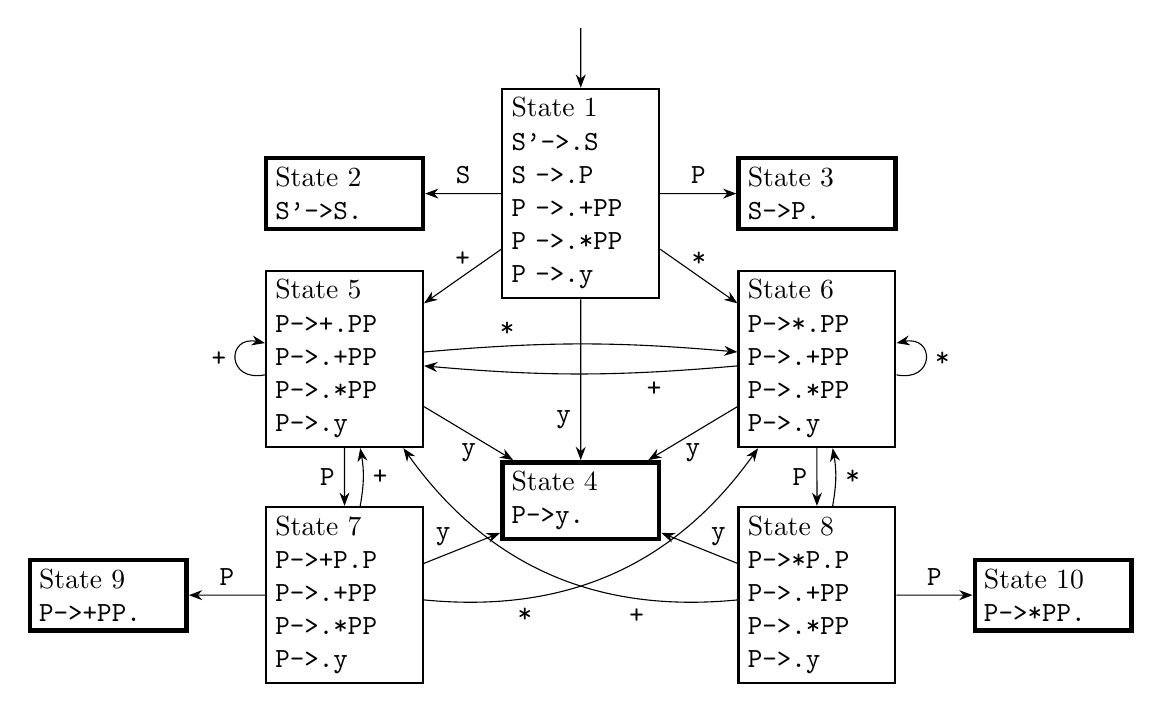
\begin{tikzpicture}[scale=3, >=Stealth,
   state/.style={rectangle, text width=50, thick},
   final/.style={ultra thick}]
   \node (q1) at (3,6) [draw, state] {State 1\\
\texttt{S'->.S}\\
\texttt{S ->.P}\\
\texttt{P ->.+PP}\\
\texttt{P ->.*PP}\\
\texttt{P ->.y}};
   \node (q2) at (2, 6) [draw, state, final] {State 2\\
\texttt{S'->S.}};
   \node (q3) at (4, 6) [draw, state, final] {State 3\\
\texttt{S->P.}};
   \node (q4) at (3, 4.7) [draw, state, final] {State 4\\
\texttt{P->y.}};
   \node (q5) at (2, 5.3) [draw, state] {State 5\\
\texttt{P->+.PP}\\
\texttt{P->.+PP}\\
\texttt{P->.*PP}\\
\texttt{P->.y}};
   \node (q6) at (4, 5.3) [draw, state] {State 6\\
\texttt{P->*.PP}\\
\texttt{P->.+PP}\\
\texttt{P->.*PP}\\
\texttt{P->.y}};
   \node (q7) at (2, 4.3) [draw, state] {State 7\\
\texttt{P->+P.P}\\
\texttt{P->.+PP}\\
\texttt{P->.*PP}\\
\texttt{P->.y}};
   \node (q8) at (4, 4.3) [draw, state] {State 8\\
\texttt{P->*P.P}\\
\texttt{P->.+PP}\\
\texttt{P->.*PP}\\
\texttt{P->.y}};
   \node (q9) at (1, 4.3) [draw, state, final] {State 9\\
\texttt{P->+PP.}};
   \node (q10) at (5, 4.3) [draw, state, final] {State 10\\
\texttt{P->*PP.}};
   \draw (3,6.7)[->] -- (q1);
   \draw (q1)[->] -- node[above]{\texttt{S}} (q2);
   \draw (q1)[->] -- node[above]{\texttt{P}} (q3);
   \draw (q1)[->] -- node[left, near end]{\texttt{y}} (q4);
   \draw (q1)[->] -- node[above]{\texttt{+}} (q5);
   \draw (q1)[->] -- node[above]{\texttt{*}} (q6);
   \draw (q5)[->] .. controls ++(-0.5, -0.1) and ++(-0.5, +0.1) .. node[left]{\texttt{+}} (q5);
   \draw (q5)[->] -- node[below]{\texttt{y}} (q4);
   \draw [->] (q5) to [bend left=5] node[above, near start]{\texttt{*}} (q6);
   \draw (q5)[->] -- node[left]{\texttt{P}} (q7);
   \draw (q6)[->] -- node[below]{\texttt{y}} (q4);
   \draw [->] (q6) to [bend left=5] node[below, near start]{\texttt{+}} (q5);
   \draw (q6)[->] .. controls ++(0.5, -0.1) and ++(0.5, +0.1) ..  node[right]{\texttt{*}} (q6);
   \draw (q6)[->] -- node[left]{\texttt{P}} (q8);
   \draw [->] (q7) to node[above, near start]{\texttt{y}} (q4);
   \draw [->] (q7) to [bend right=10] node[right]{\texttt{+}} (q5);
   \draw [->] (q7) to [bend right=30] node[below, near start]{\texttt{*}} (q6);
   \draw (q7)[->] -- node[above]{\texttt{P}} (q9);
   \draw [->] (q8) to node[above, near start]{\texttt{y}} (q4);
   \draw [->] (q8) to [bend left=30] node[below, near start]{\texttt{+}} (q5);
   \draw [->] (q8) to [bend right=10] node[right]{\texttt{*}} (q6);
   \draw (q8)[->] -- node[above]{\texttt{P}} (q10);

\end{tikzpicture}
\end{document}
